\documentclass[11pt,a4paper]{article}
\usepackage[utf8]{inputenc}
\usepackage{ngerman}
\usepackage{amsmath}
\usepackage{amsfonts}
\usepackage{amssymb}
\usepackage{graphicx}
\usepackage{tikz}
\usetikzlibrary{arrows, automata, positioning}
\begin{document}
	\title{Übung Nr.1 zur Vorlesung IPI}
	\author{David Bubeck und Patrick Nisble}
	\maketitle
	\section{''Fahrkartenautomat''}
		\begin{figure}[h]
			\centering
			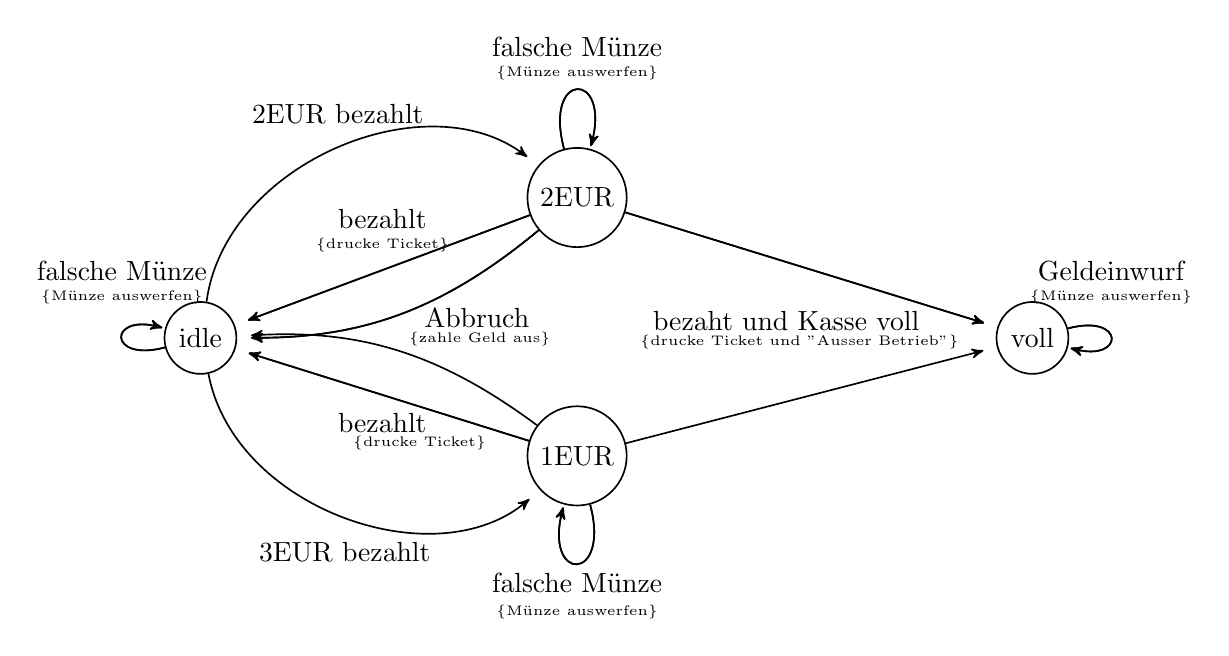
\begin{tikzpicture}[->, >=stealth', shorten >=5pt, semithick]
			
				\node [state]  	(1)											{idle};
				\node [state]	(21)	[above right = 1cm and 4cm of 1]	{2EUR};
				\node [state]	(22)	[below = 2cm of 21]					{1EUR};
				\node [state]	(3)		[below right = 1cm and 5cm of 21]	{voll};
				
				\path	(1)	edge [loop left] 		node[above=.6cm] {falsche Münze} 			(1)
							edge [loop left]		node[above=.3cm] {\tiny \{Münze auswerfen\}} (21)
				
							edge [bend left=60] 	node [above=.2cm] {2EUR bezahlt} 	(21)
							
							edge [bend right=60]	node [below=.2cm] {3EUR bezahlt}	(22)
				
						(21) edge [loop above] 			node[above=.3cm] {falsche Münze}(21)
							edge [loop above]				node[above] {\tiny \{Münze auswerfen\} } 		(21)
				
							edge [bend left = 20] 	node [below right = -.2cm and .2cm] {Abbruch} 				(1)
							edge [bend left = 20]	node [below right = .1cm and 0] {\tiny \{zahle Geld aus\}}	(1)
				
							edge [bend left = 0] 	node [above=.4cm] {bezahlt} 				(1) 
							edge [bend left = 0]	node [above=.1cm] {\tiny \{drucke Ticket\}} 	(1)
							
							edge [above]			node [below left = .4cm and -1.5cm] {bezaht und Kasse voll}(3)
							edge [below]			node [below left = .7cm and -2cm] {\tiny \{drucke Ticket und ''Ausser Betrieb''\}} (3)
							
						(22) edge [loop below] 		node[below] {falsche Münze}(21)
							edge [loop below]		node[below=.4cm] {\tiny \{Münze auswerfen\} } 		(21)
							edge [bend right = 20] 	node {} 				(1)
						
							edge [bend right = 0] 	node [below=.1cm] {bezahlt} 				(1) 
							edge [bend right = 0]	node [below right =.4cm and -.5cm] {\tiny \{drucke Ticket\}} 	(1)
							
							edge [above]			node {}(3)
							
						(3)	edge [loop right]		node[above=.6cm] {Geldeinwurf}	(3)
							edge [loop right]		node[above=.3cm] {\tiny \{Münze auswerfen\}} (3)
				;
			
			\end{tikzpicture}
			
			\caption{Fahrkartenautomat, m: Momentanbetrag, n = Sollbetrag}
			\label{fig:f1}
		\end{figure}
	\newpage
	\section{Automat: ''Bibliothek''}
		\begin{figure}[h]
			\centering
			
			\begin{tabular}{c | p{2.5cm} p{2.5cm} p{2.5cm} p{4cm}}
				&	neues Buch	&	Buch abgeben	&	Buch ausleihen 	&	Ausleihfrist abgelaufen	\\ \hline
									
				Grundzustand	&	\tiny Buch wird katalogisiert und ist ausleihbar	& - &	\tiny ''Buch nicht verfügbar''	& -	\\
				
				
			\end{tabular}
			
			\caption{Tabellendarstelllung des Automaten}
			\label{tab:t1}
		\end{figure}
	\section{Automat für Vorfahrtsregeln}
	
		\begin{figure}[h]
			\centering
			
			\begin{tabular}{r | l l l}
				& B \& C frei & Fahrzeug an B & Fahrzeug an C \\ \hline
				heranfahren & $\rightarrow$ weiterfahren & $\rightarrow$ weiterfahren & $\rightarrow$ warten \\
				warten & $\rightarrow$ weiterfahren & - & $\rightarrow$ warten \\
			\end{tabular}			
			\caption{Übergangstabelle für A nach B}
			\label{tab:t2}
		\end{figure}
		
		\begin{figure}[h]
			\begin{tabular}{r | l l l l}
				& B \& C frei, kein F & Fahrzeug an B & Fahrzeug an C & Fahrrad \\ \hline
				heranfahren & $\rightarrow$ weiterfahren & $\rightarrow$ weiterfahren & $\rightarrow$ weiterfahren & $\rightarrow$ warten \\
				warten & $\rightarrow$ weiterfahren & - & $\rightarrow$ weiterfahren & $\rightarrow$ warten \\
			\end{tabular}			
			\caption{Übergangstabelle für A nach C}
			\label{tab:t3}
		\end{figure}
		
		\begin{figure}[h]
			\begin{tabular}{r | l l l l}
				& A \& C frei, kein F & Fahrzeug an A & Fahrzeug an C & Fahrrad \\ \hline
				heranfahren & $\rightarrow$ weiterfahren & $\rightarrow$ weiterfahren & $\rightarrow$ weiterfahren & $\rightarrow$ weiterfahren \\
				warten & $\rightarrow$ weiterfahren & $\rightarrow$ weiterfahren & $\rightarrow$ weiterfahren & $\rightarrow$ weiterfahren \\
			\end{tabular}			
			\caption{Übergangstabelle für B nach A}
			\label{tab:t4}
		\end{figure}
		
		\begin{figure}[h]
			\begin{tabular}{r | l l l l}
				& A \& C frei, kein F & Fahrzeug an A & Fahrzeug an C & Fahrrad \\ \hline
				heranfahren & $\rightarrow$ weiterfahren & $\rightarrow$ warten & $\rightarrow$ warten & $\rightarrow$ warten \\
				warten & $\rightarrow$ weiterfahren & $\rightarrow$ warten & $\rightarrow$ warten & $\rightarrow$ warten \\
			\end{tabular}			
			\caption{Übergangstabelle für B nach C}
			\label{tab:t5}
		\end{figure}
		
		\begin{figure}[h]
			\begin{tabular}{r | l l l l}
				& A \& B frei, kein F & Fahrzeug an A & Fahrzeug an B & Fahrrad \\ \hline
				heranfahren & $\rightarrow$ weiterfahren & $\rightarrow$ warten & $\rightarrow$ warten & $\rightarrow$ warten \\
				warten & $\rightarrow$ weiterfahren & $\rightarrow$ warten & $\rightarrow$ warten & $\rightarrow$ warten \\
			\end{tabular}			
			\caption{Übergangstabelle für C nach A}
			\label{tab:t6}
		\end{figure}
		
		\begin{figure}[h]
			\begin{tabular}{r | l l l l}
				& A \& B frei, kein F & Fahrzeug an A & Fahrzeug an B & Fahrrad \\ \hline
				heranfahren & $\rightarrow$ weiterfahren & $\rightarrow$ weiterfahren & $\rightarrow$ warten & $\rightarrow$ warten \\
				warten & $\rightarrow$ weiterfahren & $\rightarrow$ warten & $\rightarrow$ warten & $\rightarrow$ warten \\
			\end{tabular}			
			\caption{Übergangstabelle für C nach B}
			\label{tab:t7}
		\end{figure}
\end{document}